\documentclass[a4paper,11pt,oneside]{scrreprt}
%% Packages:
\usepackage[utf8]{inputenc}
\usepackage[T1]{fontenc}    
\usepackage{graphicx}       
\usepackage[british,UKenglish]{babel} 
\usepackage{csquotes} 
\usepackage{eurosym}
\usepackage[linktocpage=true]{hyperref} 
\usepackage{caption}
\usepackage[onehalfspacing]{setspace}
\usepackage{minted}
\usepackage[a-2b,mathxmp]{pdfx}[2018/12/22]
\usepackage[style=apa,citestyle=apa,backend=biber]{biblatex}
\addbibresource{Zotero.bib}

%% Settings:
\setcounter{secnumdepth}{4}
\setcounter{tocdepth}{4}
\captionsetup{format=hang, justification=raggedright}
\setlength{\parindent}{0pt}

% Custom Commands
\renewcommand{\listingscaption}{Listing}
\renewcommand\listoflistingscaption{List of Listings}

\begin{document}
\nocite{*}

\thispagestyle{empty}
\begin{titlepage}
  \begin{flushright}
  
\includegraphics[width=0.3\linewidth]{images/Hogeschool_van_amsterdam_logo.svg}
  \end{flushright}
  \begin{flushleft}
  \section*{Research \& Development Project}
  \subsection*{3D Dungeon Generator}

  \vspace{1cm}
  Hogeschool van Amsterdam\newline
  Gameplay Engineering

  \vspace{0.5cm}

  Michael Spiegel\newline
  \today
  \end{flushleft}
\end{titlepage}

% Table of Contents:
\tableofcontents

% Content:
\chapter{Introduction}
\label{chapter:introduction}
For my research project I chose a 3D dungeon generator that should generate a new dungeon every time the game is started. Furthermore, I decided to make it possible to explore the dungeon. For this I want to add a player that will be placed in a randomly chosen start room. To make the whole dungeon more interesting and not leave it as an empty place, I plan to add some scenery like torches and chests. Additionally the dungeon should also contain enemies for which I try to implement a combat system. The focus lies mainly on the visuals of the dungeon but the performance should also be good enough so that it is playable. As a combat system can take much time to implement and needs a lot of testing it could be possible throughout the project that I will only implement a prototype and do not keep it in the final game. Through this project I want to understand how the algorithms work that are used for dungeon generation. Furthermore, I want to get knowledge about combat systems in games.
\\
\\
The whole project can be found on \href{https://github.com/Smightym8/3DDungeonGenerator}{GitHub}.

\chapter{Research}
\label{chapter:research}

\section{Existing algorithms for dungeon generation}
\label{section:existing-algorithms}
There exist several algorithms which can be used to create dungeons. In this chapter three algorithms will be described and in the end compared. 

\subsection{Binary Space Partitioning}
\label{subsection:binary-space-partitioning}
The binary space partitioning algorithm is very popular for creating dungeons because it is a fast algorithm and not that hard to implement. With this algorithm the dungeon is represented through a binary tree structure. The initial space will be split in each iteration of the algorithm. With this algorithm it is possible to create a variety of dungeons each time the code is run. For this it is necessary that specific parts of the split have to be randomised. The split can be horizontal or vertical. Figure \ref{fig:bsp_example} shows how a dungeon generated with Binary Space Partitioning looks like. (\cite[][]{williams_investigation_nodate})

\begin{figure}[ht]
	\centering
	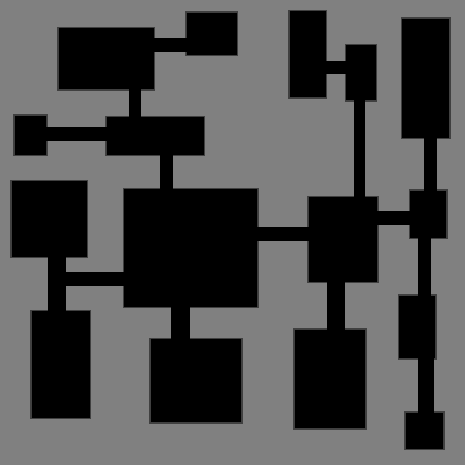
\includegraphics[scale=0.6]{images/bsp_example.png} 
	\caption{Example of a BSP generated dungeon}
	Source: \cite[][]{williams_investigation_nodate}
	\label{fig:bsp_example}
\end{figure}

\newpage
\subsection{Cellular Automata}
\label{subsection:cellular-automata}
The Cellular automata algorithm uses a grid of cells to build a dungeon. Each cell has a reference to its neighbour cells and a defined state for the time $t = 0$. With the help of predefined rules the state for $t = t + 1$ can be calculated. Depending on the defined rules and the cell states there will be patterns that occur from time to time. A cell it self represents a space where the player can walk but also a space where the player can not walk for example rocks. As you can see in figure \ref{fig:cellular_automata_example} Cellular Automata creates more cave like dungeons without real rooms. (\cite[][]{williams_investigation_nodate})

\begin{figure}[ht]
	\centering
	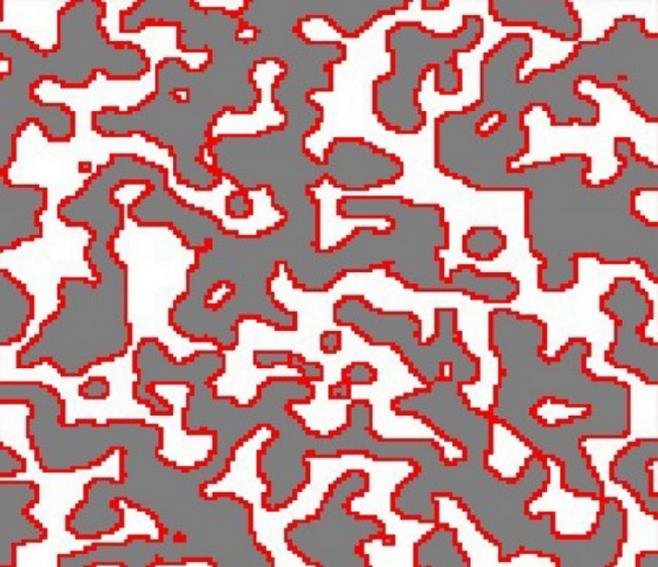
\includegraphics[scale=0.5]{images/cellular_automata_example.png} 
	\caption{Example of a Cellular Automata generated dungeon}
	Source: \cite[][]{williams_investigation_nodate}
	\label{fig:cellular_automata_example}
\end{figure}

\subsection{Delaunay Triangulation}
\label{subsection:delaunay-triangulation}
The last algorithm is the delaunay triangulation algorithm for dungeon generation. This algorithm also uses cells but in this case a random rectangle is created inside of each cell. After this step the algorithm separates the room and prevents them from overlapping. All cells that are exceeding a threshold become rooms. To connect all rooms a graph for all the room centre points is constructed. Additionally to the delaunay triangulation algorithm it is necessary to generate a minimum spanning tree of the originally create graph to remove cycles. In figure \ref{fig:delaunay_example} you can see how a dungeon generated with the delaunay triangulation looks like. Compared to the other two algorithms it is more similar to the result of the binary space partition generated dungeon because both generate square rooms. (\cite[][]{williams_investigation_nodate})

\begin{figure}[ht]
	\centering
	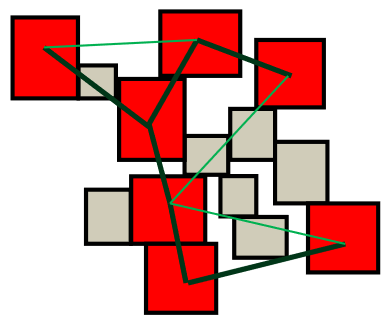
\includegraphics[scale=0.6]{images/delaunay_example.png} 
	\caption{Example of a Delaunay Triangulation generated dungeon}
	Source: \cite[][]{williams_investigation_nodate}
	\label{fig:delaunay_example}
\end{figure}

\section{Comparison of the algorithms}
\label{section:comparison-of-the-algorithms}
Now let's compare those algorithms to explain which one fits best for the purpose of this project. The cellular automata algorithm generates more cave like dungeons which is not applicable to the goal of this project. The dungeon should consist of rooms which only the binary space partition and the delaunay triangulation algorithm provides. 
\\
To compare those two algorithms let's have a look on the performance. Figure \ref{fig:bsp_performance} shows the performance of the binary space partitioning algorithm. This algorithm is slow when less rooms are used for the dungeon but has its strength in the generation of more complex dungeons that consists of a huge amount of rooms.  
\begin{figure}[ht]
	\centering
	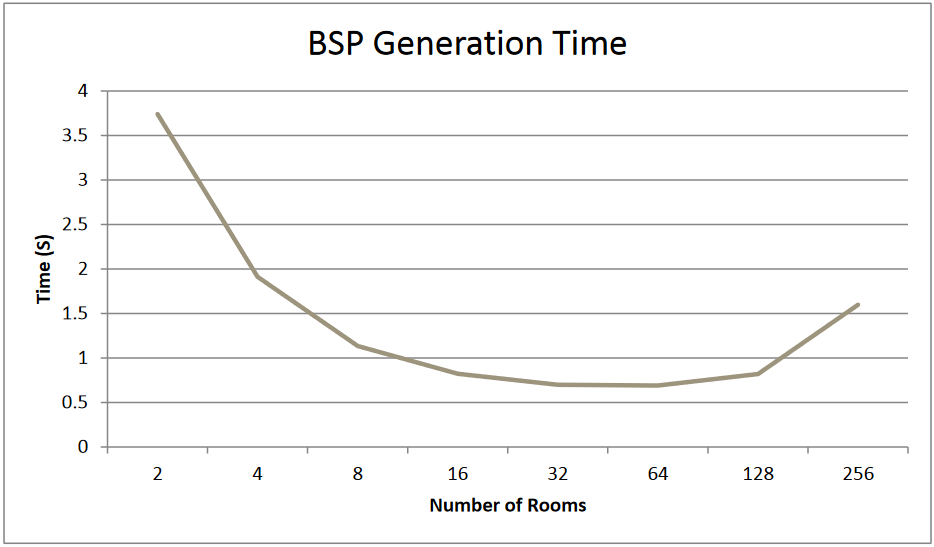
\includegraphics[scale=0.6]{images/bsp_performance.png} 
	\caption{Performance of the Binary Space Partitioning algorithm}
	Source: \cite[][]{williams_investigation_nodate}
	\label{fig:bsp_performance}
\end{figure}

\newpage
Figure \ref{fig:delaunay_performance} shows that compared to the other algorithm the delaunay triangulation algorithm is faster when it comes to dungeons with less rooms. On the other side this algorithm gets slower with the increasing amount of rooms. This means, that this algorithm fits best if the dungeon will only consist of a few rooms.
\begin{figure}[ht]
	\centering
	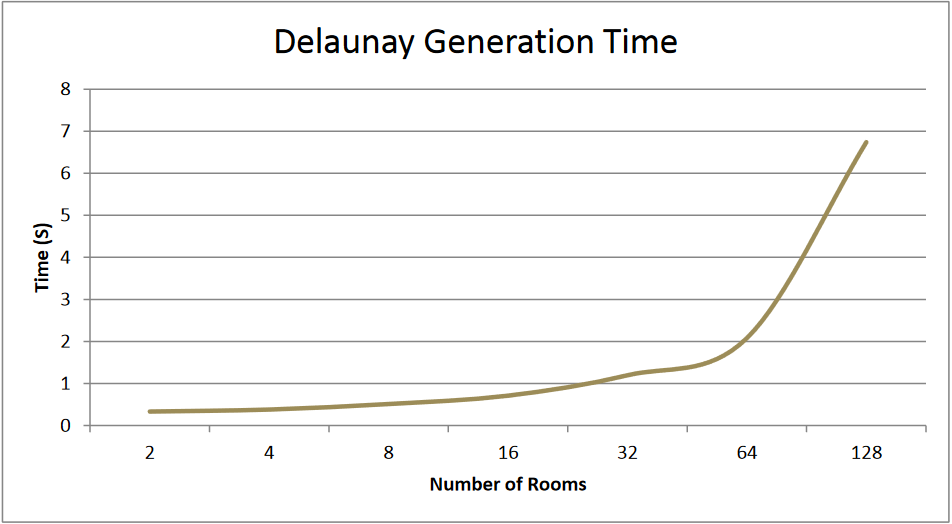
\includegraphics[scale=0.6]{images/delaunay_performance.png} 
	\caption{Performance of the Delaunay Triangulation algorithm}
	Source: \cite[][]{williams_investigation_nodate}
	\label{fig:delaunay_performance}
\end{figure}

\chapter{Implementation}
\label{chapter:implementation}
In the following sections it is shown how the generation of the dungeon has been implemented.
\section{Dungeon Generator}
\label{section:dungeon-generator}

\subsection{Creating floor and roof}
\label{subsection:creating-floor-and-roof}
\begin{figure}[ht]
	\centering
	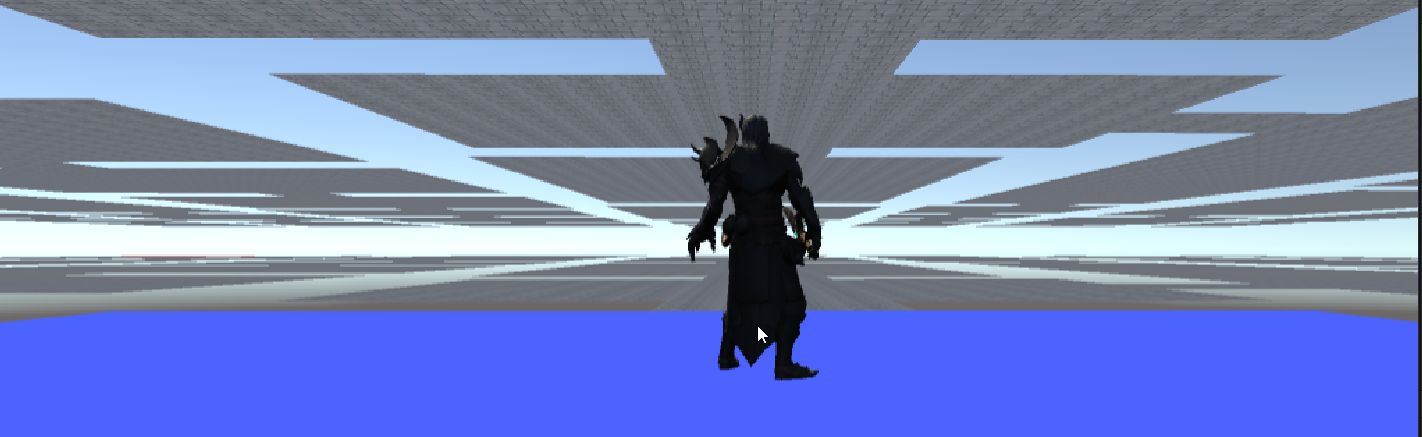
\includegraphics[scale=0.5]{images/dungeon_floor_and_roof.png}  
	\caption{Floor and roof of the dungeon}
	\label{fig:floor-roof}
\end{figure}

To create the floors the BSP algorithm is used. Before creating the meshes we need to collect all the nodes and put them in the tree structure. For this, the whole space is at first divided into two spaces and then those two are divided into another two. Each space is a node and saved in the tree structure. To decide when the space has to be divided I added a minimum and maximum for the length and width of each room. To represent the tree structure I used a queue and a list for the rooms. When a node is not between the minimum and maximum values that space will be split and the two new nodes are added to the queue and list. The orientation of the room is selected randomly or based on the length and width of the room. So not all rooms are horizontal or vertical.
\\
\\
After collecting all the nodes, we have to find all the lowest leafs because those have to be drawn as rooms. To find them the tree is traversed until the lowest leaves are reached. Each room node has two corner points and the other two can be calculated with the help of the existing ones. 
\\
\\
To finally create a mesh for each room we have to loop through all the room nodes. The same nodes can also be used for the roof because it is the same with a different height. As you can see the creation of the triangles is also different. As each room is a rectangle with four corners we can draw two triangles to get a rectangle mesh.
\\
\\
To create the corridors each node is connected with its neighbour node. The corridor nodes are handled like room nodes and therefore also stored in the same list that we use to iterate over. The mesh creation is also the same.
\\
\begin{listing}[ht]
    \inputminted[fontsize=\footnotesize,linenos]{csharp}{code/CreateFloorRoof.cs}
    \caption[Creation of floor and roof]{Creation of floor and roof}
    \label{code:creation-of-floor-and-roof}
\end{listing}

\newpage
\subsection{Determining Start and end room}
\label{subsection:determining-start-and-end-room}
To find the start room it is not much work necessary. I only check the index while iterating over the list of rooms and choose the first created room as start room. 

\begin{figure}[ht]
	\centering
	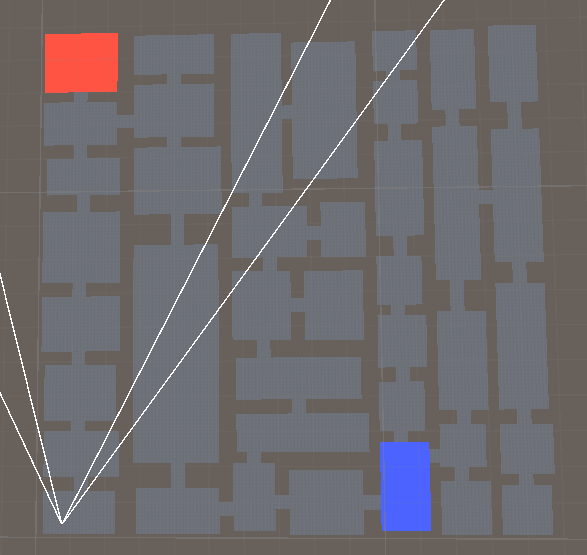
\includegraphics[scale=0.5]{images/start_end_room.png}   
	\caption{Start room (blue) and end room (red)}
	\label{fig:start-end-room}
\end{figure}

For the end room I thought about which rooms could be end rooms and I think the best case is when the end room is not too near to the start room. For this I calculate the distance between each room and the start room. The room that is the furthest away will be the end room.
\\
\begin{listing}[ht]
    \inputminted[fontsize=\footnotesize,linenos]{csharp}{code/EndRoom.cs}
    \caption[Determining end room]{Determining end room}
    \label{code:Determining-end-room}
\end{listing}

\subsection{Creating walls}
\label{subsection:creating-walls}
\begin{figure}[htb]
	\centering
	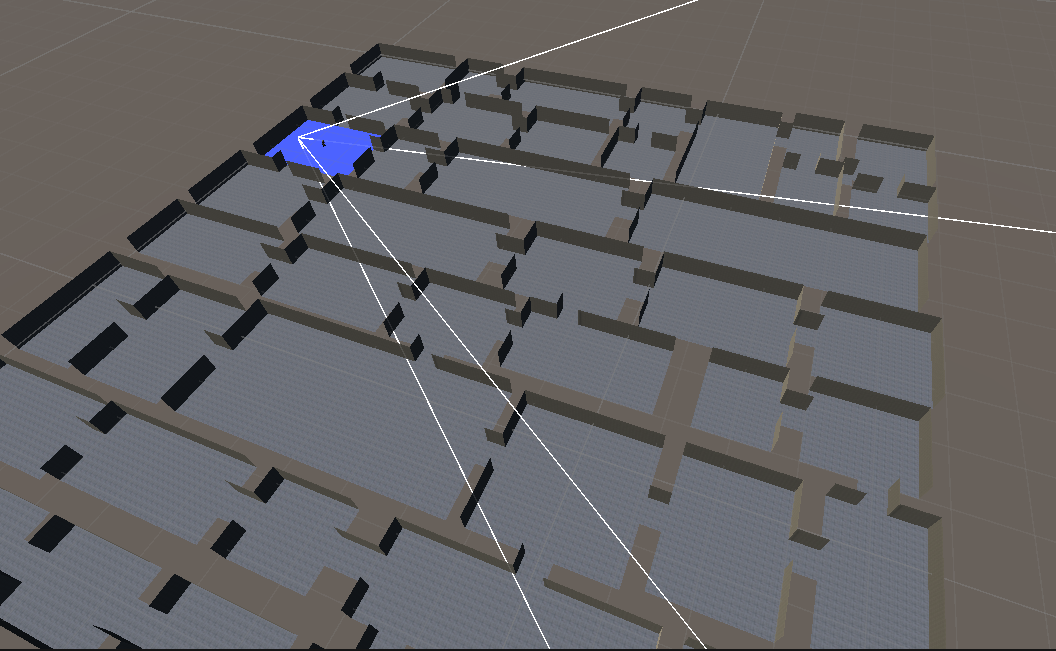
\includegraphics[scale=0.4]{images/walls.png}   
	\caption{Walls of the dungeon}
	\label{fig:walls}
\end{figure}

The creation of the rooms got a bit complicated because of the corridors. For each side of the room it is checked if the corners of the corridor are between the corners of that side of the room. If that is the case, the wall has to be divided into two walls. The corners of the corridor act then once as end point and once as start point for the two walls. If there is no corridor the wall can be created for the whole length of that room side. The corridors only get walls on two sides so they are open to walk through. In figure \ref{fig:detecting-corridors-between-room-corners} you can see that the two walls will be created from roomStart to corridorStart and from corridorEnd to roomEnd.
\begin{figure}[htb]
	\centering
	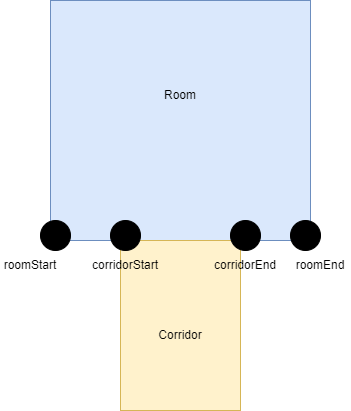
\includegraphics[scale=0.49]{images/detecting_corridors.drawio.png}    
	\caption{Detecting corridors between room corners}
	\label{fig:detecting-corridors-between-room-corners}
\end{figure}

There is also a special case for creating the walls when the corridor is not placed between the room corners. Figure \ref{fig:detecting-corridors-at-room-corners} shows how it looks like when the corridors are placed the the corner of the room. Depending on the room corner the walls have to be created from corridorStart to roomStart and from corridorEnd to roomEnd or from roomStart to corridorStart and from roomEnd to corridorEnd.

\begin{figure}[htb]
	\centering
	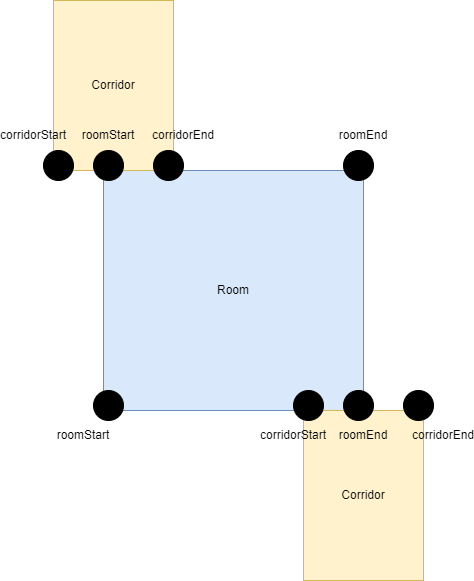
\includegraphics[scale=0.49]{images/detecting_corridors2.drawio.png}    
	\caption{Detecting corridors at room corners}
	\label{fig:detecting-corridors-at-room-corners}
\end{figure}

Before creating the mesh it is necessary to get the positions of the vertices. This works like the creation of a plane but instead of creating it flat, it has to be created into the y direction. Depending on the direction of the wall it will be created into the x and y direction or the z and y direction. Horizontal walls use the x direction and vertical walls the z direction. 
\\
\\
Creating the mesh is very simple. The only difference compared to a plane in this case is, that I have to check if it is a horizontal or vertical wall for the calculation of the length. It is also important to flip the creation of the vertices. 
All walls have to be visible from the inside of the rooms and therefore the triangles can not be created the same way for all walls. Some walls need the triangles to be drawn clock wise and some counter clockwise.
\\
\begin{listing}[ht]
    \inputminted[fontsize=\footnotesize,linenos]{csharp}{code/CreateWalls3.cs}
    \caption[Creating wall mesh]{Creating wall mesh}
    \label{code:creating-wall-mesh}
\end{listing}

\newpage
\subsection{Lighting}
\label{subsection:lighting}
\begin{figure}[htb]
	\centering
	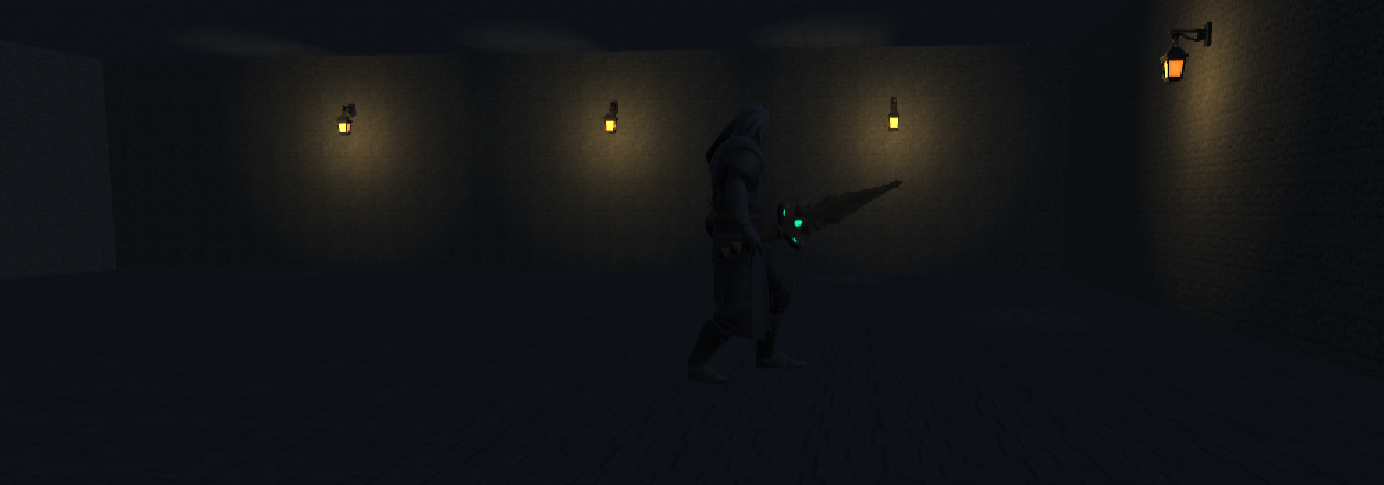
\includegraphics[scale=0.45]{images/lights.png}   
	\caption{Lights in the dungeon}
	\label{fig:lights}
\end{figure}
To get the positions for the lights the length of the wall is calculated and divided by the frequency of the lights. With the help of steps it will be decided if that position is used for the lights. For corridors the wall positions are ignored because with this approach it would always place the maximum amount of lights per wall. To prevent that the open space of the corridor is used to place lights, only that sides of it are used for collection the positions.
\\
\\
As positions can occur multiple times because of overlapping between walls, It is checked if a point is already in the list for the possible positions. If that is the case the position will be removed and added to another list to ignore that positions in the future. To keep track over all points I used two lists, one for the possible positions and one list for the actual positions. For the actual positions it depends if isGettingLight is true. Additionally to the position the rotation is added so the light prefabs are all facing inside the room. 
\begin{listing}[ht]
    \inputminted[fontsize=\footnotesize,linenos]{csharp}{code/Lights2.cs}
    \caption[Saving light positions]{Saving light positions}
    \label{code:saving-light-positions}
\end{listing}

\newpage
\subsection{Combining meshes}
\label{subsection:combining-meshes}
This method is from the \href{https://docs.unity3d.com/ScriptReference/Mesh.CombineMeshes.html}{Unity documentation}. It is slightly modified and uses a parent as input parameter and a boolean to check if it is a wall or a floor/roof. 
\\
Depending on the boolean it assigns the appropriate material and layer. The layer is needed for the third person camera of the player. Furthermore the mesh collider is added after combining the meshes.

\subsection{Placing scenery}
\label{subsection:placing-scenery}
To place the scenery I iterate over all rooms except the start room. To prevent that multiple sceneries are placed at the same position, the position is added to a list. While placing the scenery it checks if the position is already in use and generates a new position if this is the case. Furthermore all the sceneries will be rotated towards the centre point of the room.
\begin{listing}[ht]
    \inputminted[fontsize=\footnotesize,linenos]{csharp}{code/Scenery.cs}
    \caption[Rotating scenery]{Rotating scenery}
    \label{code:rotating-scenery}
\end{listing}

\section{Combat system}
\label{section:combat-system}
I implemented a prototype for the combat system and asked my classmates and friends if they can test it and give me feedback. As the combat system was not matching my criteria to prevent the player from running through the dungeon and ignoring the visuals I decided to not put further work in it. The feedback was also not that good because a combat system needs much work and the focus during my project is not about the combat system. Nevertheless I want to show how I implemented my prototype.

\subsection{Player}
\label{subsection:player}
The player can start to attack with clicking the left mouse button. If the player attacks an enemy it will call a method of the script health that is attached to the enemy. The enemy will then start attacking the player. It is also possible that the enemy attacks the player without being attacked by the player before. 
\begin{listing}[ht]
    \inputminted[fontsize=\footnotesize,linenos]{csharp}{code/Player.cs}
    \caption[Player attack]{Player attack}
    \label{code:player-attack}
\end{listing}

\subsection{Enemy}
\label{subsection:enemy}
The enemy has three states:
\begin{itemize}
\item Patroling
\item Chasing
\item Attacking
\end{itemize}

In the first state, the enemy is walking around to a random destination point within the navigation mesh. The enemy enters the second state when the player is in a specific range and starts running towards the player. After the enemy reached the player the attacking state is activated and the enemy starts attacking.
\begin{listing}[ht]
    \inputminted[fontsize=\footnotesize,linenos]{csharp}{code/Enemy.cs}
    \caption[Enemy movement states]{Enemy movement states}
    \label{code:enemy-movement-states}
\end{listing}

\section{Core game mechanic: Finding the key}
\label{section:core-game-mechanic}
As the focus of the project lies on the visuals and one of my initial goals was to create a little game where the generated dungeon is used, I decided to let the player search a key in the dungeon. With the key it is possible to open a door that has to be found as well. Through the door the next level can be reached. With searching the key the player is forced to look around while exploring the dungeon. This should lead to recognizing the visuals more.
\\
\\
The table with the key, that is necessary to open the door, is placed in the middle of a random chosen room. The door is placed in the end room. Determining that room was explained in section \ref{subsection:determining-start-and-end-room} on page \pageref{subsection:determining-start-and-end-room}. To prevent that the door is placed in front of a corridor the methods for the wall creation are used to check if the wall borders on a corridor. The door will then be placed in a wall that does not border a corridor.

\chapter{Conclusion and Outlook}
\label{chapter:conclusion-and-outlook}

\section{Conclusion}
\label{section:conclusion}
I learned really much throughout the last few weeks. In the end the whole dungeon is generated including the walls which were prefabs at first. My understanding for procedural content generation is now much better than before the project. Beside the generation of the dungeon I also took a look on combat systems and implemented one but unfortunately it did not match my criteria because it would have needed much more work.  
\\
\\
In general I learned a lot about developing in Unity for example adding lights, show messages through a trigger and many other things as I did not have that much experience before. Furthermore there was also a bit of game design and user testing while implementing the combat system. I think for the period of five weeks I did a good work.

\section{Outlook}
\label{section:outlook}
For the future there is still so much that can be done about this project. It would be possible to put more effort into the combat system and make the search for the key more difficult. Another thing that is still not completely finished is the game mechanic, here I would like to add more than one key per level. For this it would also be cool if the player would be able to set marks which will be displayed on the mini map to mark the door if it is found before all the keys. I have many ideas and hope that I can continue my work on that topic in the future.

% List of Figures:
\clearpage
\phantomsection
\addcontentsline{toc}{chapter}{List of Figures}
\listoffigures

% List of Listings:
\clearpage
\phantomsection
\addcontentsline{toc}{chapter}{List of Listings}
\listoflistings

% Bibliography:
\clearpage
\phantomsection
\addcontentsline{toc}{chapter}{Bibliography}
\printbibliography
\end{document}